\section{Bootware Core Library}

We have seen in \autoref{design:flow} and \autoref{design:finalarch} that the local and remote bootware have some common functionality.
It would make sense to implement these components in such a way that they can share this common functionality.
This would avoid code duplication and make changes to common functionality easier.
Therefore, we introduce the bootware core library, which will encapsulate the common functionality of both bootware components.

\begin{figure}[!htbp]
	\centering
	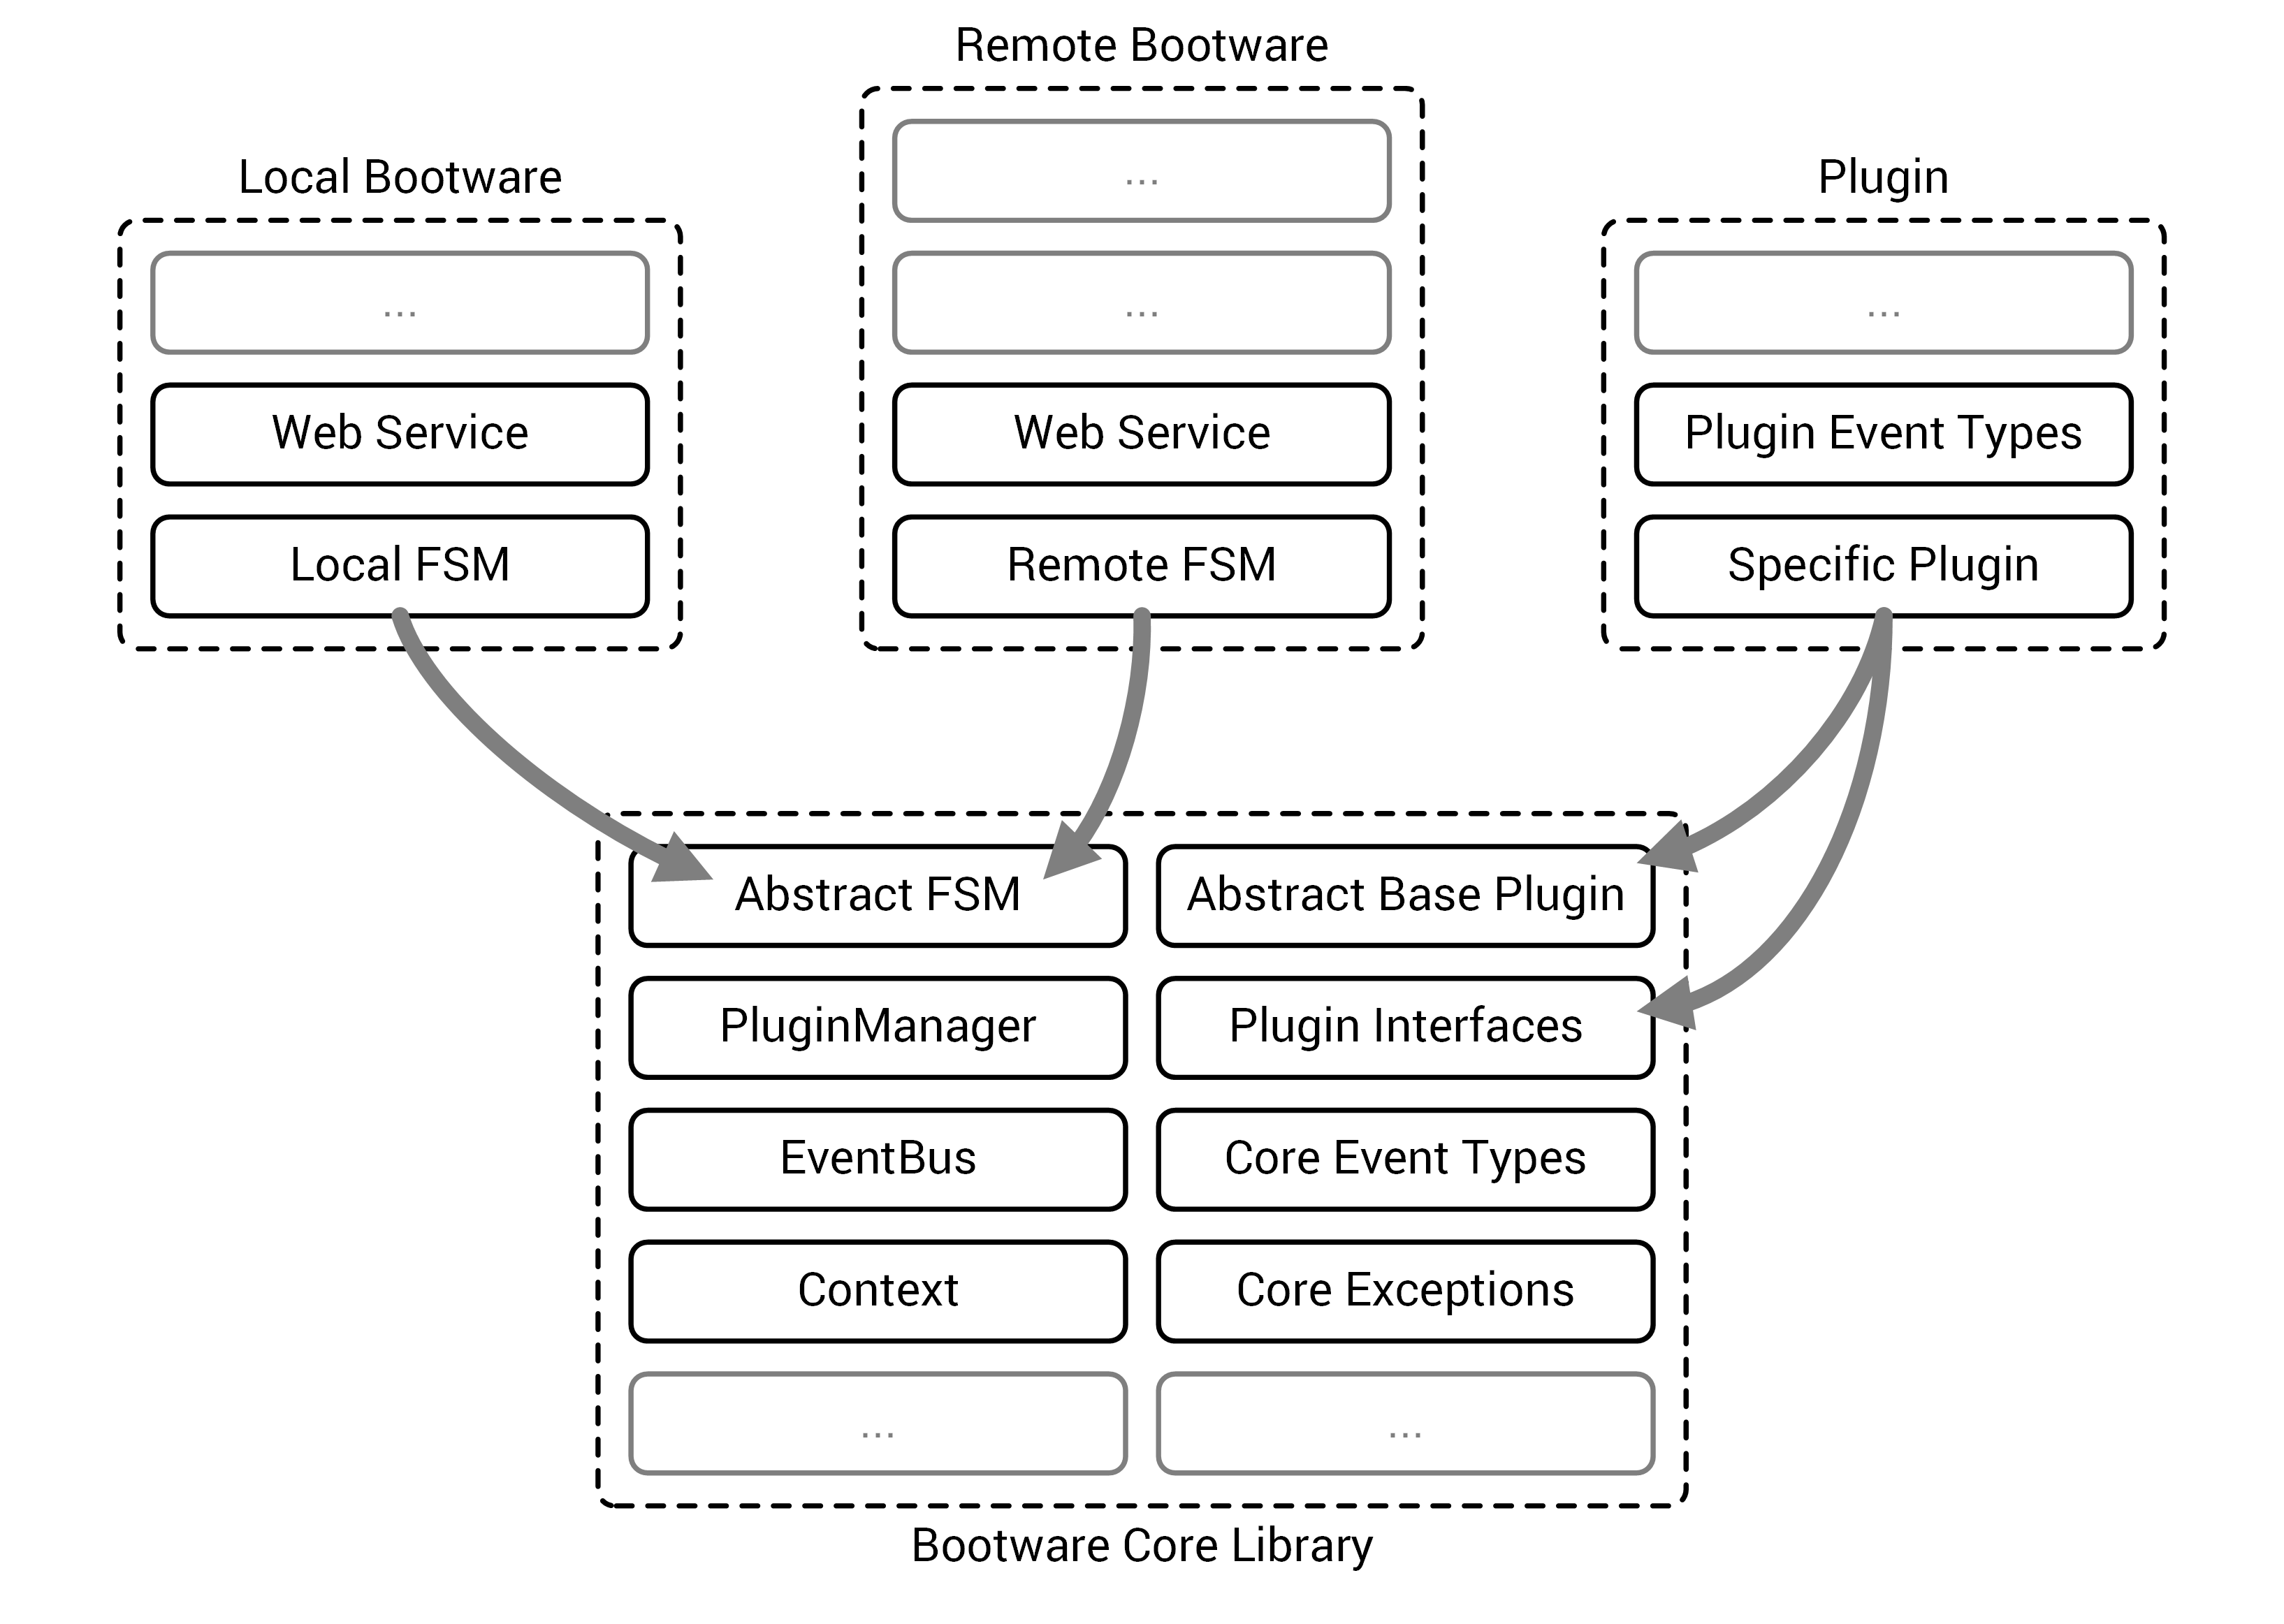
\includegraphics[resolution=600]{implementation/assets/core_library}
	\caption{The bootware core library and exemplary usage.}
	\label{image:corelibrary}
\end{figure}

Because we are using Java for the implementation, the core library will be a \textit{.jar} file containing common classes that will be imported by the local and remote bootware implementations and also by plugin implementations.
\autoref{image:corelibrary} shows a schematic view of the bootware core library and how its classes are used by various components.
We can see that the library includes an abstract FSM class, which is used by both the local and the remote bootware implementation.
The abstract FSM class defines common state machine functionality that is used by both bootware components.
This includes function definitions for the shared states shown in \autoref{image:flow_local} and \autoref{image:flow_remote}.
This way, the local and remote bootware can import shared states from the library and only have to define their custom states (e.g. the provision middleware states in the remote bootware or the send to remote state in the local bootware) and the state transitions.
They can also overwrite the states imported from the library if this is necessary.

The library also includes an abstract base plugin class, which implements some functionality that is common to all plugin.
Actual plugin implementations can extend this base plugin class to inherit this common functionality.
They also have to implement one of the plugin interfaces defined in the bootware core library, so for example, a resource plugin has to implement the resource plugin interface.

Aside from the code imported from the bootware core library, the components using the library are free to add various other code to their implementation.
This way, the remote bootware could implement some extra functionality not needed in the local bootware, or a plugin could define its own event types.
